The introductory section sets us up nicely to discuss the coveted reproducing kernel Hilbert space.
This is a subset of Hilbert spaces for which its evaluation functionals are continuous (by definition, in fact).
The majority of this section, apart from defining RKHS, is an exercise in convincing ourselves that each and every RKHS of functions can be specified solely through its reproducing kernel.
To begin, we consider a fundamental linear functional on a Hilbert space of functions $\cF$, that assigns a value to $f \in \mathcal F$ for each $x \in \mathcal X$, called the \emph{evaluation functional}.

%\begin{figure}[htb]
%  \centering
%  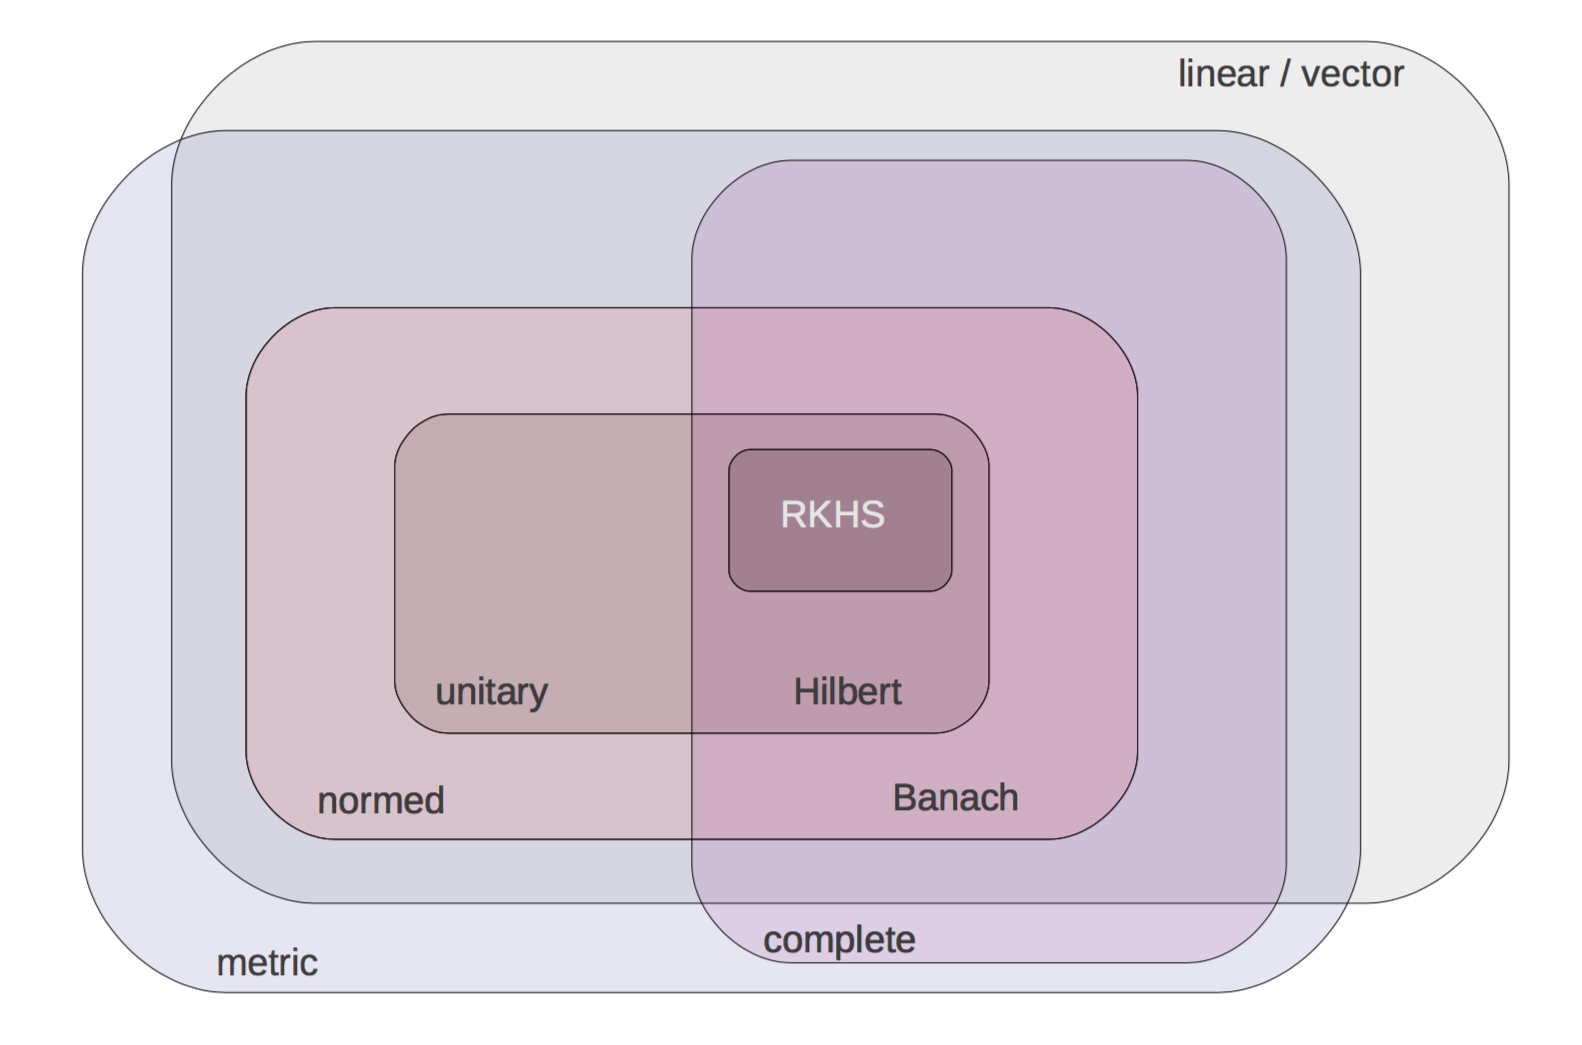
\includegraphics[width=0.75\textwidth]{figure/02-hierarchy-spaces.png}
%  \caption[A hierarchy of vector spaces]{A hierarchy of vector spaces\footnotemark.}
%\end{figure}
%\footnotetext{Reproduced from the lecture slides of Dino Sejdinovic and Arthur Gretton entitled `Foundations of Reproducing Kernel Hilbert Spaces: Advanced Topics in Machine Learning', 2014. URL: \url{http://www.stats.ox.ac.uk/~sejdinov/teaching/atml14/Theory_slides2_2014.pdf}.}

\definecolor{DOLLARBILL}{HTML}{89C168}
\definecolor{IGUANA}{HTML}{6AC38C}
\definecolor{AUROMETALSAURUS}{HTML}{6A8482}
\definecolor{FLAME}{HTML}{ED5324}
\definecolor{PASTELBROWN}{HTML}{836A54}
\definecolor{CHINESERED}{HTML}{9A3D23}
\definecolor{MYWHITE}{HTML}{F5EDEB}

\begin{figure}
  \centering
  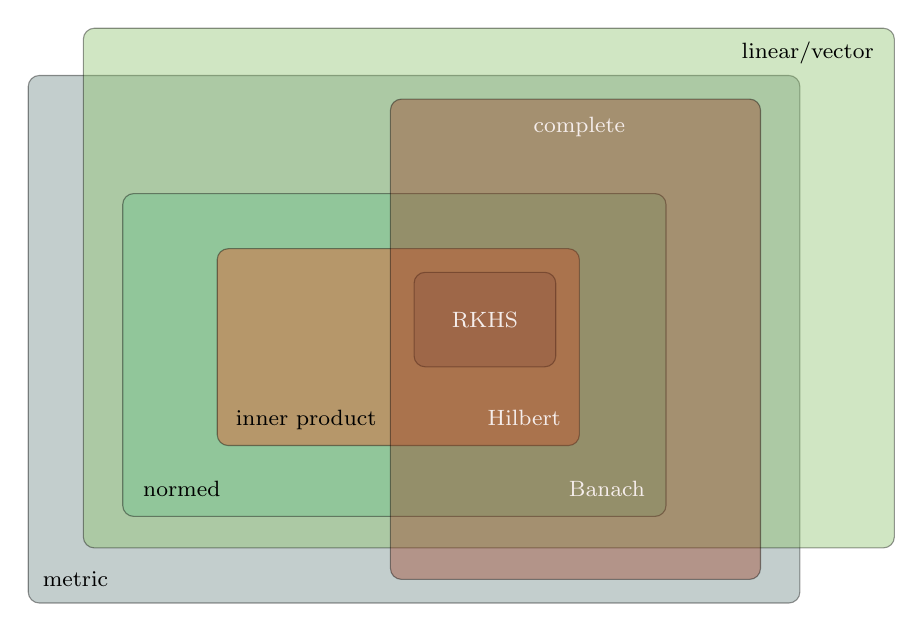
\begin{tikzpicture}
  
    \draw[rounded corners,fill=AUROMETALSAURUS,opacity=0.4] (0,0) rectangle (9.8,6.7);  % metric
    \draw[rounded corners,fill=DOLLARBILL,opacity=0.4] (0.7,0.7) rectangle (11,7.3);  % vector
    \draw[rounded corners,fill=IGUANA,opacity=0.4] (1.2,1.1) rectangle (8.1,5.2);  % normed
    \draw[rounded corners,fill=FLAME,opacity=0.4] (2.4,2) rectangle (7,4.5);  % inner product
    \draw[rounded corners,fill=PASTELBROWN,opacity=0.4] (4.9,3) rectangle (6.7,4.2);  % RKHS
    \draw[rounded corners,fill=CHINESERED,opacity=0.4] (4.6,0.3) rectangle (9.3,6.4);  % complete
    
    \node[draw=none,text=MYWHITE,align=center] at (5.8,3.6) {\footnotesize RKHS};
    \node[draw=none,text=black] at (0.6,0.3) {\footnotesize metric};
    \node[draw=none,text=black] at (1.95,1.45) {\footnotesize normed};
    \node[draw=none,text=MYWHITE] at (7.35,1.45) {\footnotesize Banach};
    \node[draw=none,text=black] at (3.53,2.32) {\footnotesize inner product};
    \node[draw=none,text=MYWHITE] at (6.3,2.35) {\footnotesize Hilbert};
    \node[draw=none,text=MYWHITE] at (7,6.05) {\footnotesize complete};
    \node[draw=none,text=black] at (9.9,6.98) {\footnotesize linear/vector};
    
  \end{tikzpicture}
  \caption[A hierarchy of vector spaces]{A hierarchy of vector spaces\footnotemark.}
\end{figure}
\footnotetext{Reproduced from the lecture slides of Dino Sejdinovic and Arthur Gretton entitled `Foundations of Reproducing Kernel Hilbert Spaces: Advanced Topics in Machine Learning', 2014. URL: \url{http://www.stats.ox.ac.uk/~sejdinov/teaching/atml14/Theory_slides2_2014.pdf}.}


\begin{definition}[Evaluation functional]
	Let $\mathcal F$ be a vector space of functions $f:\mathcal X \rightarrow \mathbb R$, defined on a non-empty set $\mathcal X$. 
	For a fixed $x \in \mathcal X$, the functional $\delta_x:\mathcal F \rightarrow \mathbb R$ as defined by $\delta_x(f) = f(x)$ is called the (Dirac) evaluation functional at $x$.
\end{definition}

It is easy to see that evaluation functionals are always linear: $\delta_x(\lambda f + g) = (\lambda f + g)(x) = \lambda f(x) + g(x) = \lambda\delta_x(f) + \delta_x(g)$ for $\lambda\in\bbR$, $f,g\in\cF$ real functions over $\cX$.
Humble as they may seem, the entirety of the evaluation functionals over the domain $\cX$ determines $f$ uniquely and thus are of great importance in understanding the space $\cF$.
Core topological properties like convergence are hinged on continuity, and it is therefore important that evaluation functionals are continuous.
As it turns out, RKHSs by definition provide exactly this.

\begin{definition}[Reproducing kernel Hilbert space]\label{def:rkhs}
	A Hilbert space $\cF$ of real-valued functions $f:\mathcal X \rightarrow \mathbb R$ on a non-empty set $\mathcal X$ is called a \emph{reproducing kernel Hilbert space} if the evaluation functional $\delta_x: f \mapsto f(x)$ is continuous (equivalently, bounded) on $\cF$, $\forall x \in \cX$. 
\end{definition}

Continuity (boundedness) of evaluation functionals in an RKHS means that functions that are close in RKHS norm imply that they are also close pointwise, since $\vert \delta_x(f) - \delta_x(g) \vert = \vert \delta_x(f-g) \vert \leq M\Vert f-g \Vert_\cF$ for some real $M>0$.
Note that the converse is not necessarily true.
RKHSs are particularly well behaved in this respect, compared to other Hilbert spaces, and this property in particular has desirable consequences for a wide variety of applications, including nonparametric curve estimation, learning and decision theory, and many more.

%This gives some reassurance when estimating $f$ from $\cF$ using the the norm of the space as a criterion for selection.
%More formally,
%\begin{corollary}[Norm convergence implies pointwise convergence in RKHS]\label{thm:normpointconv}
%  Let $\cF$ be an RKHS of real functions over $\cX$, and let $f_n$ be a sequence of points in $\cF$.
%  Then, for some $f\in\cF$,
%  \[
%    \lim_{n\to\infty} \norm{f_n - f}_\cF = 0 \ \ \Rightarrow \ \ \lim_{n\to\infty} |f_n(x) - f(x)| = 0.
%  \]
%\end{corollary}
%
%\begin{proof}
%  Suppose $\cF$ is an RKHS with reproducing kernel $h$.
%  Then,
%  \begin{align*}
%    \vert \delta_x(f) - \delta_x(g) \vert
%    &= \vert \delta_x(f-g) \vert \\
%    &= \vert (f-g)(x) \vert  \\
%    &= \vert \ip{f-g,h(\cdot,x)}_\cF \vert \mycomment{(reproducing property)} \\
%    &\leq \norm{h(\cdot,x)}_\cF \cdot \norm{f-g}_\cF \mycomment{(Cauchy-Schwarz)} \\
%    &= \sqrt{h(x,x)}\cdot \norm{f-g}_\cF. \qedhere
%  \end{align*}
%\end{proof}
%
%\begin{figure}[t]
%  \centering
%  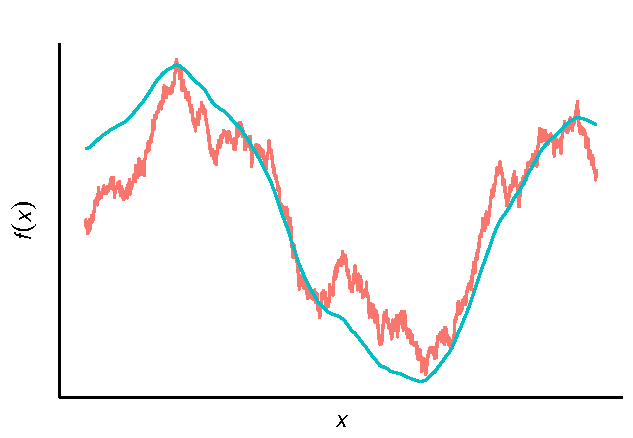
\includegraphics[width=0.7\textwidth]{figure/02-conv_in_norm}
%  \caption[Pointwise closeness does not imply closeness in norm.]{In a RKHS, two functions which are close together in norm are close pointwise, but the converse is not necessarily true. Functions which appear to be close to each other may actually diverge with respect to the norm of the RKHS.}
%\end{figure}

%The continuity condition also represents the weakest condition required for both the existence of an inner product and the evaluation of every function in $\cF$ at every point in the domain $\cX$.
While the continuity condition by definition is what makes an RKHS, it is neither easy to check this condition in practice, nor is it intuitive as to the meaning of its name.
In fact, there isn't even any mention of what a reproducing kernel actually is.
In order to benefit from the desirable continuity property of RKHS, we should look at this from another, more intuitive, perspective. 
By invoking the Riesz representation theorem, we see that for all $x\in\cX$, there exists a unique element $h_x\in\cF$ such that
\[
  f(x) = \delta_x(f) = \ip{f,h_x}_\cF, \forall f \in \cF
\]
holds. 
Since $h_x$ itself is a function in $\cF$, it holds that for every $x' \in \cX$ there exists a $h_{x'}\in\cF$ such that
\[
  h_{x}(x') = \delta_{x'}(h_{x}) = \ip{h_x,h_{x'}}_\cF.
\]
This leads us to the definition of a \emph{reproducing kernel} of an RKHS---the very notion that inspires its name.

\begin{definition}[Reproducing kernels]\label{def:repkern}
  Let $\mathcal F$ be a Hilbert space of functions over a non-empty set $\mathcal X$. 
  A symmetric, bivariate function $h:\mathcal X\times\mathcal X\rightarrow\mathbb R$ is called a \emph{kernel}, and it is a \emph{reproducing kernel} of $\mathcal F$ if $h$ satisfies
  \begin{itemize}
    \item $\forall x \in \mathcal X,\, h(\cdot, x) \in \mathcal F$; and
    \item $\forall x \in \mathcal X, \, f \in \mathcal F, \, \langle f, h(\cdot, x) \rangle_{\mathcal F} = f(x)$ (the reproducing property).
  \end{itemize}
  In particular, for any $x, x' \in \mathcal X$,
  \[
  	h(x,x') = \langle h(\cdot, x), h(\cdot, x') \rangle_{\mathcal F}.
  \]
\end{definition}

An important property for reproducing kernels of a RKHS is that they are positive-definite functions.
That is, $\forall a_1, \dots, a_n \in \mathbb R$ and $\forall x_1, \dots, x_n \in \mathcal X$,
\[
  \sum_{i=1}^n\sum_{j=1}^n a_i a_j h(x_i, x_j) \geq 0.
\]

\begin{claim}[Reproducing kernels of RKHS are positive-definite]\label{thm:posdef}
  Let $\hXXR$ be a reproducing kernel for a Hilbert space $\cF$.
  Then $h$ is a symmetric and positive definite function.
\end{claim}

\begin{proof}
  \begin{align*}
    \sum_{i=1}^n\sum_{j=1}^n a_i a_j h(x_i, x_j)	
    &= \sum_{i=1}^n\sum_{j=1}^n a_i a_j \langle  h(\cdot, x_i), h(\cdot, x_j) \rangle_{\mathcal F} \displaybreak[1] \\
    &= \Bigg\langle \sum_{i=1}^n a_i h(\cdot, x_i), \sum_{j=1}^n a_j h(\cdot, x_j) \Bigg\rangle_{\mathcal F} \\
    &= \Bigg\Vert \sum_{i=1}^n a_i h(\cdot, x_i) \Bigg\Vert_{\mathcal F}^2 \\
    & \geq 0 \qedhere
  \end{align*}
\end{proof}

\begin{remark}
  In the kernel method literature, a \emph{kernel} $\hXXR$ is usually defined as the inner product between inputs in feature space.
  That is, take $\phi:\cX\to\cV$, $x\mapsto\phi(x)$, where $\cV$ is a Hilbert space.
  Then the kernel is defined as $h(x,x') = \ip{\phi(x),\phi(x')}_\cV$, for any $x,x'\in\cX$.
  The space $\cV$ is known as the \emph{feature space} and the mapping $\phi$ the \emph{feature map}.
  In many mathematical models involving feature space mappings, elucidation of the feature map and feature space is not necessary, and thus computation  is made simpler by the use of kernels (known as the \emph{kernel trick}---\cite{hofmann2008kernel}).
  Note that kernels defined in this manner are positive definite, while in this thesis, we opt for a more general definition allowing kernels to not necessarily be positive.
  The relevance of this generality will be appreciated when we discuss reproducing kernel Kreĭn spaces in \cref{sec:rkkstheory}.
\end{remark}

Introducing the following definition of the \emph{kernel matrix} (also known as the \emph{Gram matrix}) is useful at this point.
\begin{definition}[Kernel matrix]
  Let $\{x_1,\dots,x_n\}$ be a sample of points, where each $x_i\in\cX$, and $h$ a kernel over $\cX$.
  Define the \emph{kernel matrix} $\bH$ for $h$ as the $n \times n$ matrix with $(i,j)$ entries equal to $h(x_i,x_j)$.
\end{definition}
Obviously, $\bH$ is a positive-definite matrix if the kernel that defines it is positive-definite: $\ba^\top\bH\ba = \sum_{i=1}^n\sum_{j=1}^n a_ia_jh(x_i,x_j) \geq 0$ for any choice of $a_1,\dots,a_n\in\bbR$ and $x_1,\dots,x_n\in\cX$.

So far, we have seen that reproducing kernels of a RKHS are positive-definite functions, and that RKHSs are Hilbert spaces with continuous evaluation functionals, but one might wonder what exactly the relationship between a reproducing kernel and a RKHS is.
%there are several questions we might like the answer to: What is the relationship between a reproducing kernel and an RKHS? Can we speak to its existence and uniqueness? What other properties does it have?
We assert the following:
\begin{itemize}
  \item \textbf{RKHS $\Leftrightarrow$ reproducing kernel} (\cref{{thm:rkhsunique}}). For every RKHS $\cF$ of functions over a set $\cX$, there corresponds a unique, positive-definite reproducing kernel $\hXXR$, and vice-versa. That is, a Hilbert space is a RKHS if it possesses a unique, reproducing kernel.
  \item \textbf{P.d. function $\Rightarrow$ RKHS} (\cref{{thm:moorea}}). For every positive-definite function $\hXXR$, there corresponds a unique RKHS $\cF$ that has $h$ as its reproducing kernel.
\end{itemize}
In essence, the notion of positive-definite functions and reproducing kernels of a RKHS are equivalent, and that there is a bijection between the set of positive-definite kernels and the set of RKHSs.
The rest of this section is a consideration of these assertions, addressed by the two theorems that follow.

\begin{theorem}[RKHS uniqueness]\label{thm:rkhsunique}
  Let $\cF$ be a Hilbert space of functions over $\cX$.
  $\cF$ is a RKHS if and only if $\cF$ has a reproducing kernel $\hXXR$, and that $h$ is unique to $\cF$.
\end{theorem}

\begin{proof}
  First we tackle existence, i.e., we prove that $\cF$ is a RKHS if and only if $\cF$ has a reproducing kernel.
  Suppose $\cF$ is a Hilbert space of functions, and $\hXXR$ is a reproducing kernel for $\cF$.
  Then, choosing $\delta=\epsilon / \norm{h(\cdot,x)}_\cF$, for any $f \in \cF$ such that $\norm{f-g}_\cF < \delta$, we have
  \begin{align*}
    \vert \delta_x (f) - \delta_x (g) \vert 
    &= \vert (f-g)(x) \vert \\
    &= |\ip{f-g,h(\cdot,x)}_\cF| \mycomment{(reproducing property)} \\
    &\leq \norm{h(\cdot,x)}_\cF \cdot \norm{f-g}_\cF \mycomment{(Cauchy-Schwarz)} \\
    &= \epsilon.
  \end{align*}
  Thus, the evaluation functional is (uniformly) continuous on $\cF$, and by definition, $\cF$ is a RKHS.
  Now suppose that $\cF$ is a RKHS, and $h$ is a kernel function over $\cX\times\cX$.
  The reproducing property of $h$ is had by following the argument preceding \cref{def:repkern}.
 
  As for uniqueness, assume that the RKHS $\cF$ has two reproducing kernels $h_1$ and $h_2$. 
  Then, $\forall f\in\cF$ and $\forall x\in\cX$,
  \begin{align*}
    \ip{f,h_1(\cdot,x) - h_2(\cdot,x)}_\cF = f(x) - f(x) = 0.
  \end{align*}
  In particular, if we take $f = h_1(\cdot,x) - h_2(\cdot,x)$, we obtain $\norm{h_1(\cdot,x) - h_2(\cdot,x)}^2_\cF = 0$.
  Thus, $h_1=h_2$.
\end{proof}

\begin{theorem}[Moore-Aronszajn]\label{thm:moorea}
  If $\hXXR$ is a positive-definite function then there exists a unique RKHS whose reproducing kernel is $h$.
\end{theorem}

\begin{proof}[Sketch proof]
  Most of the details here have been omitted, except for the parts which we feel are revealing as to the properties of an RKHS.
  For a complete proof, see \citet{berlinet2011reproducing}. 
  Start with the linear space
  \[
    \cF_0 = \left\{ f_n:\cX\to\bbR \, \Big| \, f_n = \sum_{i=1}^n w_i h(\cdot,x_i), x_i\in\cX, w_i\in\bbR, n\in\bbN \right\}
  \]
  and endow this linear space with the following inner product:
  \[\label{eq:rkhsinnerprod}
    \left\langle \sum_{i=1}^n w_i h(\cdot,x_i), \sum_{j=1}^m w_j' h(\cdot,x_j') \right\rangle_{\cF_0} = \sum_{i=1}^n\sum_{j=1}^m w_i w_j' h(x_i,x_j').
  \]
  It may be shown that this indeed a valid inner-product satisfying the conditions laid in \cref{def:innerprod}.
  At this point, the reproducing property is already had:   \begin{align*}
    \big\langle f_n, h(\cdot,x) \big\rangle_{\cF_0} 
    &= \left\langle \sum_{i=1}^n w_i h(\cdot,x_i), h(\cdot,x) \right\rangle_{\cF_0} \\
    &= \sum_{i=1}^n w_i h(x_i,x) \\
    &= f_n(x),
  \end{align*}
  for any $f_n\in\cF_0$.
  
  Let $\cF$ be the completion of $\cF_0$ with respect to this inner product.
  In other words, define $\cF$ to be the set of functions $f:\cX\to\bbR$ for which there exists a Cauchy sequence $\{f_n\}_{n=1}^\infty$ in $\cF_0$ converging pointwise to $f \in \cF$.
  The inner product for $\cF$ is defined to be
  \[
    \ip{f,f'}_\cF = \lim_{n\to\infty} \ip{f_n,f_n'}_{\cF_0}.
  \]
  The sequence $\{ \ip{f_n,f_n'}_{\cF_0} \}_{n=1}^\infty$ is convergent and does not depend on the sequence chosen, but only on the limits $f$ and $f'$ \citep[Lemma 5]{berlinet2011reproducing}.
  We may check that this indeeds defines a valid inner product.
  The reproducing property carries over to the completion:
  \begin{align*}
    \ip{f,h(\cdot,x)}_\cF 
    &= \lim_{n\to\infty} \ip{f_n,h(\cdot,x)}_{\cF_0} \\
    &= \lim_{n\to\infty} f_n(x) \\
    &= f(x).
  \end{align*}
  
  To prove uniqueness, let $\cG$ be another RKHS with reproducing kernel $h$.
  $\cF$ has to be a closed subspace of $\cG$, since $h(\cdot,x) \in \cG$ for all $x\in\cX$, and because $\cG$ is complete and contains $\cF_0$ and hence its completion.
  Using the orthogonal decomposition theorem, we have $\cG = \cF \oplus \cF^\bot$, i.e. any $g\in\cG$ can be decomposed as $g = f + f^c$, $f\in\cF$ and $f^c\in\cF^\bot$.
  For each element $g\in\cG$ we have that, for all $x\in\cX$,
  \begin{align*}
    g(x) &= \ip{g,h(\cdot,x)}_\cG \\
    &= \big\langle f+f^c, h(\cdot,x) \big\rangle_\cG \\
    &= \big\langle f, h(\cdot,x) \big\rangle_\cG + \cancelto{0}{\big\langle f^c, h(\cdot,x) \big\rangle_\cG} \\
    &= f(x)
  \end{align*}
  so therefore $g\in\cF$ too.
  It must be that $\cF\equiv\cG$.
  %$\cF\cong\cG$.
%  
%  Minor detail: $f^c \in \cF^\bot \Rightarrow f^c \in \{f\in\cF | \ip{f,f'} = 0 \ \forall f'\in\cF \}$. Thus
%  \begin{align*}
%    \big\langle f^c, h(\cdot,x) \big\rangle_\cG 
%    &= f^c(x) \\
%    &= \big\langle f^c, h(\cdot,x) \big\rangle_\cF \\
%    &= 0
%  \end{align*}
%  It is evident that the inner product as defined is symmetric, linear, and positive-definite due to the positive-definiteness of reproducing kernels.
%  The only non-trivial condition to check is that whether $\ip{f_n,f_n}_{\cF_0}$ implies $f_n=0$.
%  To see this, realise that
%  \begin{align*}
%    0 &\leq 
%    1
%  \end{align*}
%  
%  By the Cauchy-Schwarz inequality, we see that
%  \begin{align*}
%    |f_n(x)| &= \big| \big\langle f_n, h(\cdot,x) \big\rangle_{\cF_0} \big| \\
%    &\leq \Vert h(\cdot,x) \Vert_{\cF_0} \cdot \Vert f_n \Vert_{\cF_0}    \\
%    &= \sqrt{h(x,x)} \cdot \Vert f_n \Vert_{\cF_0}
%  \end{align*}
%  so convergence in norm implies pointwise convergence.
%  By a similar argument in the proof of \cref{thm:normpointconv}, we also get that pointwise convergence is implied by convergence in norm for this space.
%  In particular, for every Cauchy sequence $\{f_n\}_{n=1}^\infty$ in $\cF_0$, $\big\{f_n(x)\big\}_{n=1}^\infty$ is a Cauchy sequence on the real line.
%  Complete the space $\cF_0$ by adjoining all of these limits to it, and call this completed space $\cF$.
%  
%  Furthermore, note that $\big\vert \norm{f_n}_{\cF_0} - \norm{f_m}_{\cF_0} \big\vert \leq \norm{f_n - f_m}_{\cF_0}$ (triangle inequality), so for a Cauchy sequence $\{f_n\}_{n=1}^\infty$ in a complete space, $\norm{f_n}_{\cF_0}$ has a limit.
%  Define the norm of $\cF$ to be $\norm{f}_\cF = \lim_{n\to\infty} \norm{f_n}_{\cF_0}$ for any $f\in\cF$.
%  Next, extend the inner product from $\cF_0$ to $\cF$ by defining $\ip{f,g}_\cF = \lim_{n\to\infty} \langle f_n,g_n \rangle_{\cF_0}$, where
%  \[
%    \lim_{n\to\infty} \langle f_n,g_n \rangle_{\cF_0} = \lim_{n\to\infty} \half\left( \norm{f+g}_{\cF_0}^2 - \norm{f}_{\cF_0}^2 - \norm{g}_{\cF_0}^2\right).
%  \]
%  One can indeed verify this is a well-defined inner product.
\end{proof}

A consequence of the above proof is that we can show that any function $f$ in a RKHS $\mathcal F$ with kernel $h$ can be written in the form $f(x) = \sum_{i=1}^n h(x, x_i)w_i$, with some $(w_1,\dots,w_n)\in\bbR^n$, $n \in \mathbb N$. 
More precisely, $\mathcal F$ is the completion of the space $\mathcal G = \text{span}\{h(\cdot,x) \, | \, x \in \mathcal X \}$ endowed with the inner product as stated in \cref{eq:rkhsinnerprod}.



